
\usetikzlibrary{arrows}

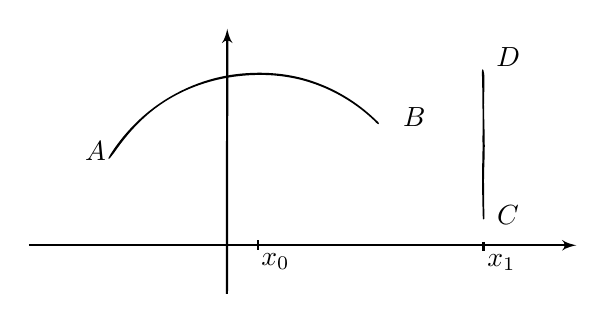
\begin{tikzpicture}[y=0.80pt, x=0.8pt,yscale=-1,scale=0.3, inner sep=0pt, outer sep=0pt]
\begin{scope}[shift={(220.0315,-356.64289)}]% layer1
  \begin{scope}[shift={(3147.7678,-1427.0496)}]% g1988
    % path2584-0-9
    \path[draw=black,line join=miter,line cap=butt,line width=0.800pt,-latex']
      (-3367.7993,2109.6489) -- (-2543.3619,2109.6489);

    % path2582-4-4
    \path[draw=black,line join=miter,line cap=butt,line width=0.800pt,-latex']
      (-3069.5306,2182.6982) -- (-3068.9608,1783.6932);

  \end{scope}
  % path2010
  \path[cm={{1.0,0.0,0.0,-1.0,(3140.5045,2591.4389)}},color=black,fill=black,line
    width=0.800pt] (-3235.0518,2049.7501) .. controls (-3224.7011,2065.1961) and
    (-3212.8770,2079.6329) .. (-3199.6736,2092.6944) .. controls
    (-3185.8590,2106.3606) and (-3170.5392,2118.5216) .. (-3154.0121,2128.7327) ..
    controls (-3141.0975,2136.7119) and (-3127.5595,2143.6755) ..
    (-3113.5002,2149.4165) .. controls (-3092.3728,2158.0428) and
    (-3070.0886,2163.9194) .. (-3047.4083,2166.5846) .. controls
    (-3036.9248,2167.8165) and (-3026.3793,2168.5155) .. (-3015.8188,2168.6123) ..
    controls (-3002.0742,2168.7382) and (-2988.3043,2167.8430) ..
    (-2974.6857,2165.8204) .. controls (-2961.0670,2163.7979) and
    (-2947.6000,2160.6459) .. (-2934.5389,2156.2799) .. controls
    (-2928.9138,2154.3996) and (-2923.3554,2152.3245) .. (-2917.8777,2150.0571) ..
    controls (-2888.1454,2137.7477) and (-2860.8772,2119.7384) ..
    (-2837.9127,2097.4492) .. controls (-2835.8085,2095.8616) and
    (-2834.4951,2094.4459) .. (-2833.8004,2093.3682) .. controls
    (-2833.1057,2092.2905) and (-2833.0283,2091.5492) .. (-2833.3979,2091.2668) ..
    controls (-2833.7675,2090.9844) and (-2834.5829,2091.1593) ..
    (-2835.6950,2091.8948) .. controls (-2836.8072,2092.6302) and
    (-2838.2149,2093.9250) .. (-2839.8065,2095.8845) .. controls
    (-2862.6019,2117.7680) and (-2889.6013,2135.3976) .. (-2918.9552,2147.3999) ..
    controls (-2924.1566,2149.5268) and (-2929.4302,2151.4786) ..
    (-2934.7636,2153.2533) .. controls (-2947.7980,2157.5905) and
    (-2961.2382,2160.6999) .. (-2974.8212,2162.6755) .. controls
    (-2988.4042,2164.6511) and (-3002.1297,2165.4952) .. (-3015.8188,2165.3238) ..
    controls (-3025.6539,2165.2008) and (-3035.4728,2164.5543) ..
    (-3045.2376,2163.4448) .. controls (-3056.3564,2162.1815) and
    (-3067.7159,2160.2127) .. (-3079.0244,2157.4677) .. controls
    (-3090.3328,2154.7226) and (-3101.5880,2151.2009) .. (-3112.4932,2146.9331) ..
    controls (-3126.9193,2141.2882) and (-3140.7121,2134.3204) ..
    (-3153.3148,2126.4801) .. controls (-3161.6745,2121.2795) and
    (-3169.4669,2115.6340) .. (-3176.8031,2109.6323) .. controls
    (-3184.1393,2103.6306) and (-3191.0206,2097.2722) .. (-3197.5570,2090.5778) ..
    controls (-3209.2352,2078.6173) and (-3219.8315,2065.6124) ..
    (-3229.8529,2051.2471) .. controls (-3231.8245,2048.4895) and
    (-3234.9274,2044.3105) .. (-3237.2789,2041.4877) .. controls
    (-3238.4547,2040.0763) and (-3239.4528,2039.0115) .. (-3240.0687,2038.6716) ..
    controls (-3240.6845,2038.3317) and (-3240.9230,2038.7196) ..
    (-3240.5412,2040.2037) .. controls (-3239.2798,2043.2106) and
    (-3237.0488,2046.6938) .. (-3235.0518,2049.7501) -- cycle;

  % path2032
  \path[draw=black,line join=miter,line cap=butt,line width=0.800pt]
    (124.5441,675.1125) -- (124.5441,689.1781);

  % text2036
  \path[fill=black] (130.17809,718.74866) node[above right] (text2036) {$x_0$};

  \begin{scope}[shift={(2906.3668,-1422.8206)}]% g1992
  \end{scope}
  % path2040
  \path[fill=black] (462.1640,423.4449) .. controls (462.8869,441.4579) and
    (462.7591,459.4976) .. (463.0949,477.5536) .. controls (463.4306,495.6095) and
    (462.9294,513.6809) .. (463.1058,531.7551) .. controls (463.2821,549.8292) and
    (462.1360,567.9062) .. (462.3806,585.9739) .. controls (462.6252,604.0413) and
    (462.9609,622.0995) .. (463.5014,640.1357) .. controls (462.3453,645.1237) and
    (467.2841,644.7979) .. (465.9389,639.9897) .. controls (465.5684,622.1183) and
    (465.4085,604.2244) .. (465.3263,586.3227) .. controls (465.2441,568.4209) and
    (466.5393,550.5115) .. (466.4796,532.6091) .. controls (466.4199,514.7066) and
    (465.6750,495.1342) .. (465.3719,477.2607) .. controls (465.0687,459.3872) and
    (466.5077,443.2139) .. (465.6953,425.3991) .. controls (465.4684,422.1464) and
    (464.1545,415.4341) .. (462.4766,418.2293) .. controls (462.0479,419.7616) and
    (462.1372,421.7163) .. (462.1640,423.4449) -- cycle;

  % path2032-8
  \path[draw=black,line join=miter,line cap=butt,line width=0.800pt]
    (464.6885,677.6608) -- (464.6885,691.7264);

  % text2036-5
  \path[fill=black] (470.32239,721.29706) node[above right] (text2036-5) {$x_1$};

  % text928
  \path[shift={(-220.0315,354.3321)},fill=black] (84.882782,200.68317) node[above
    right] (text928) {$A$};

  % text932
  \path[shift={(-220.0315,354.3321)},fill=black] (563.47406,149.20039) node[above
    right] (text932) {$B$};

  % text936
  \path[fill=black] (484.98737,651.64496) node[above right] (text936) {$C$};

  % text940
  \path[fill=black] (483.79834,413.49042) node[above right] (text940) {$D$};

\end{scope}

\end{tikzpicture}

